\documentclass[../main.tex]{subfiles}
\begin{document}
Chương trình bày về mục đích và các giải pháp tồn tại cho hệ thống, phân tích ưu nhược điểm các phương pháp từ đó đề xuất mô hình mới giải quyết hạn chế phương pháp trước đó; thiết kế, thử nghiệm mô hình và đánh giá kết quả. 
\section{Đề xuất}
\subsection{Mục đích hệ thống}
Hệ thống được xây dựng với mục đích:
\begin{enumerate}
    \item Cung cấp dịch vụ sinh số ngẫu nhiên có thể kiểm chứng được cho khách hàng đảm bảo an toàn, không ai có thể thao túng.
    \item Hệ thống cung cấp dịch vụ liên tục.
    \item Thu phí sử dụng dịch vụ sinh số ngẫu nhiên và trả phần thưởng cho các bên tham gia cung cấp.
\end{enumerate}
Ngoài ra hệ thống được thiết kế phải đảm bảo thời gian phản hồi không quá lâu. Thử nghiệm thành công trên mạng thử nghiệm Ethereum.
\subsection{Các giải pháp đã tồn tại}
Trong phần này em xin trình bày về các giải pháp hiện nay đang áp dụng, từ đó phân tích ưu và nhược điểm.
Đa số các dApps nhỏ đều sử dụng blockhash như là nguồn ngẫu nhiên cho dịch vụ của mình. Với cơ chế đồng thuận bằng chứng công việc hiện nay, blockhash mang tính không dự đoán trước. Tuy nhiên blockhash bị các thợ đào (miner) kiểm soát. Các thợ đào có thể đảo thứ tự các transaction rồi tìm mã băm cho tới khi được kết quả như ý mới công bố lên mạng blockchain.

Với việc tiềm ẩn rủi ro về hệ thống nhưng các ứng dụng phi tập trung này vẫn sử dụng blockhash như là nguồn cấp ngẫu nhiên là do:
\begin{enumerate}
    \item Chi phí lấy nguồn ngẫu nhiên rẻ.
    \item Độ khó khi thợ đào được một block mới tăng cao trong bối cảnh thị trường tiền ảo tăng cao, thu hút nhiều thợ đào. Khiến thợ giảm khả năng đào được block mới và tăng tiền thưởng khuyến khích trung thực.
\end{enumerate}

Do vậy ...

Chain Link là gã khổng lồ tiên phong trong việc cung cấp nguồn ngẫu nhiên có thể kiểm chứng có trả phí.
\begin{figure}[h!]
    \centering
    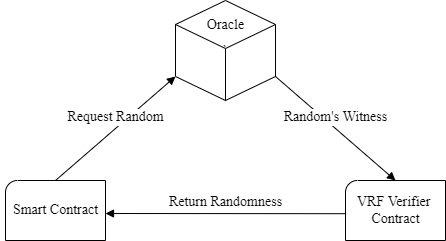
\includegraphics[scale = 0.8]{Figure/flow_chainLink.png}
    \caption{Cách hoạt động của ChainLink}
    \label{fig:flow_chainLink}
\end{figure}

Mô hình hoạt động của ChainLink được mô tả tổng quát trong hình \ref{fig:flow_chainLink}. Mô hình hoạt động theo luồng như sau. Mỗi khi hợp đồng thông minh yêu cầu một số ngẫu nhiên thì sẽ phát ra một nhật ký (logs) trên blockchain. Các oracle sẽ lắng nghe các sự kiện này và sử dụng thuật toán sinh số ngẫu nhiên có thể kiểm chứng để trả về kết quả cùng bằng chứng tới một hợp đồng thông minh khác gọi là hợp đồng xác thực (VRF Verifier Contract). Nếu hợp đồng xác thực bằng chứng cùng kết quả là khớp sẽ trả số ngẫu nhiên về cho hợp đồng yêu cầu ban đầu. 

Cho đến hiện tại Chainlink đã phát hành hai phiên bản dịch vụ  sinh số ngẫu nhiên có thể kiểm chứng trên mạng blockchain. Với phiên bản thứ nhất, Chainlink yêu cầu người dùng cung cấp cho Oracle một số ngẫu nhiên (seed) để làm dữ liệu đầu vào. Sau đó thực hiện theo luồng được mô tả trên hình \ref{fig:flow_chainLink}. Cách thiết kế này sẽ đảm bảo được:
\begin{enumerate}
    \item Người dùng không thể biết trước được kết quả ngẫu nhiên.
    \item Oracle không thể biết trước kết quả cho đến khi người dùng cung cấp seed.
    \item Oracle phải đưa ra bằng chứng hợp lệ không gian lận.
\end{enumerate}

Tuy nhiên trong phiên bản thứ nhất, đứng trên trải nghiệm người dùng, phải cung cấp cho Oracle một số để làm yếu tố đầu vào sẽ gây phức tạp tới quy trình sử dụng dịch vụ. 

Trong phiên bản thứ hai của mình, ChainLink đã cải tiến giúp người dùng không cần phải gửi kèm một số (seed) khi yêu cầu số ngẫu nhiên mà vẫn giữ được các ưu điểm của hàm sinh số ngẫu nhiên có kiểm chứng. Bởi vì  yếu tố đầu vào sẽ được sinh ra từ địa chỉ khách hàng và blockhash của block chứa transaction yêu cầu. Điều này làm cho phía người dùng thuận tiện đơn giản hơn khi sử dụng dịch vụ. Tuy nhiên việc này lại dẫn ra một vài điểm yếu. 
\begin{enumerate}
 \item Về lý thuyết, nếu ChainLink thao túng được cả blockhash thì ChainLink hoàn toàn có thể thao túng được cả kết quả ngẫu nhiên. 
 \item Trong luồng hoạt động của mô hình này, chỉ có một Oracle đảm nhận việc sinh số ngẫu nhiên và sẽ không có gì đảm bảo việc Oracle không hoạt động trong khoảng thời gian, làm gián đoạn dịch vụ.
\end{enumerate}

Hơn nữa trong mạng Ethereum các node chỉ lưu lại blockhash của 256 block gần nhất. Chỉ cần Oracle được chỉ định sinh số ngẫu nhiên bị gián đoạn trong khoảng thời gian này thì yêu cầu khách hàng sẽ không được đáp ứng.



\subsection{Đề xuất mô hình}
Từ những hạn chế của các giải pháp đang tồn tại giải quyết bài toán sinh số ngẫu nhiên trên mạng chuỗi khối. Em đề xuất mô hình như hình \ref{fig:flow} 

\begin{figure}[h!]
    \centering
    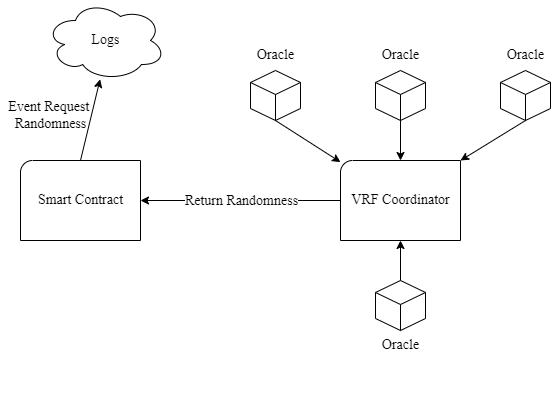
\includegraphics[scale = 0.5]{Figure/flow.png}
    \caption{Luồng mô hình sinh số ngẫu nhiên có thể kiểm chứng trên blockchain}
    \label{fig:flow}
\end{figure}

Với mỗi hợp đồng thông minh cần sử dụng số ngẫu nhiên sẽ gửi yêu cầu sinh số ngẫu nhiên. Yêu cầu này được ghi lại trên nhật ký (logs) của transaction. Mỗi Oracle nghe được yêu cầu sẽ triển khai tính toán số ngẫu nhiên kèm theo bằng chứng và trả kết quả về hợp đồng kiểm chứng VRF. Hợp đồng kiểm chứng sẽ tính toán xem liệu bằng chứng có hợp lệ hay không. Hợp đồng kiểm chứng sẽ tổng hợp các kết quả hợp lệ và gửi kết quả cuối dùng về tới cho hợp đồng khách ban đầu.

Với ý tưởng ai cũng có thể làm Oracle chỉ cần đăng ký với hợp đồng xác thực. Nếu các Oracle trung thực sẽ nhận được các phần thưởng khuyến khích. Và mô hình sẽ khắc phục được các hạn chế của phiên bản thứ hai Chainlink mà vẫn giữ được ưu điểm của hàm sinh số ngẫu nhiên có thể kiếm chứng. 
\begin{enumerate}
    \item Người có thể biết trước kết quả sinh số ngẫu nhiên thì phải sở hữu toàn bộ các Oracle, thao túng được blockhash. Rủi ro bảo mật sẽ giảm đi rất nhiều nữa nếu các bên Oracle là độc lập và tăng số lượng.
    \item Có nhiều hơn một Oracle đảm nhận việc sinh số ngẫu nhiên, do đó nếu vẫn còn đủ Oracle đạt ngưỡng đặt trước thì dịch vụ vẫn đảm bảo.
\end{enumerate}

\section{Thiết kế kiến trúc và thử nghiệm}
\subsection{Tác nhân}
Trong hệ thống này sẽ có các tác nhân như:
\begin{enumerate}
    \item Khách hàng - người sử dụng dịch vụ nhận số ngẫu nhiên có thể kiểm chứng.
    \item Người sở hữu Oracle - người đăng ký với quản lý để được cung cấp dịch vụ sinh số ngẫu nhiên.
    \item Quản lý - chủ sở hữu của dịch vụ, nhận yêu cầu từ khách hàng và phân phối tới nhà cung cấp là các Oracle. 
\end{enumerate}

\subsection{Phân tích yêu cầu chức năng và phi chức năng}
Hình \ref{fig:systemOverview} thể hiện sơ đồ trường hợp sử dụng của hệ thống (use case) của ba tác nhân: khách hàng, người sở hữu Oracle và người quản lý hợp đồng điều phối với các chức năng cơ bản.

\begin{figure}[H]
    \centering
    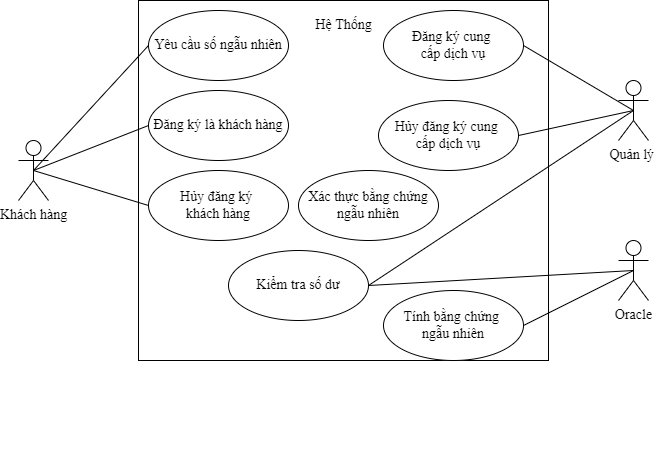
\includegraphics[scale = 0.6]{Figure/systemOverview.png}
    \caption{Sơ đồ trường hợp sử dụng của hệ thống}
    \label{fig:systemOverview}
\end{figure}


% ================================
\begin{table}[H]
\begin{tabularx}{\textwidth}{|l|X|}
Chức năng yêu cầu\\ số nhẫu nhiên:  &  \\
Mô tả:                  &Hợp đồng thông minh của khách hàng muốn gửi yêu cầu nhận số ngẫu nhiên.\\
Tác nhân:               & Khách hàng \\
Luồng cơ bản:           &
\begin{enumerate}
    \item Hợp đồng khách yêu cầu số ngẫu nhiên.
    \item Một sự kiện yêu cầu số ngẫu nhiên được phát lên nhật ký của Ethereum.
    \item Các Oracle nghe được sự kiện, sau đó tính toán bằng chứng nhẫu nhiên gửi tới hợp đồng xác thực.
    \item Hợp đồng xác thực các bằng chứng hợp lệ, tổng hợp rồi gửi về cho hợp đồng khách hàng.
    \item Hợp đồng khách hàng nhận kết quả ngẫu nhiên.
\end{enumerate}\\
Luồng ngoại lệ:         &
\begin{enumerate}
    \item Người dùng chưa đăng ký sử dụng dịch vụ sinh số ngẫu nhiên.
    \item Oracle chưa đăng ký làm bên cung cấp dịch vụ.
\end{enumerate}\\
Yêu cầu                 &\\
phi chức năng:           & 
\begin{enumerate}
    \item Thời gian trả về kết quả ngẫu nhiên không quá 10 block.
    \item Kết quả ngẫu nhiên phải được xác thực bằng chứng.
    \item Đảm bảo hợp đồng điều phối và các Oracle khó có cơ hội gian lận.
\end{enumerate}\\
\end{tabularx}
\caption{Đặc tả chức năng yêu cầu số ngẫu nhiên}
\label{table: 1}
\end{table}
Bảng \ref{table: 1} đặc tả yêu cầu chức năng sinh số ngẫu nhiên. Khách hàng phải đăng ký cho hợp đồng của mình được sử dụng dịch vụ thông qua hợp đồng điều phối (VRFCoordinator). Sau đó, transaction yêu cầu số ngẫu nhiên được công bố lên mạng chuỗi khối, các Oracle lập tức tính toán bằng chứng và gửi về cho hợp đồng điều phối. Hợp đồng điều phối xác thực bằng chứng ngẫu nhiên và gửi lại trả về cho hợp đồng khách.
% ==========================
\begin{table}[H]
\begin{tabularx}{\textwidth}{|l|X|}
Chức năng đăng ký\\ là khách hàng:  &  \\
Mô tả:                  &Hợp đồng thông minh của khách hàng muốn đăng ký sử dụng dịch vụ sinh số ngẫu nhiên.\\
Tác nhân:               & Khách hàng \\
Luồng cơ bản:           &
\begin{enumerate}
    \item Tài khoản khách hàng đăng ký cho hợp đồng sử dụng dịch vụ sinh số ngẫu nhiên.
    \item Hợp đồng điều phối (VRFCoordinator) sẽ kiểm tra địa chỉ hợp đồng khách chưa tồn tại.
    \item Tài khoản khách gửi lượng tiền làm phí dịch vụ vào hợp đồng điều phối.
    \item Số dư khả dụng để sử dụng dịch vụ của địa chỉ hợp đồng khách tăng thêm.
    \item Địa chỉ hợp đồng khách trở thành khách hàng của hợp đồng điều phối.
    \item Đăng ký thành công
\end{enumerate}\\
Luồng ngoại lệ:         &
\begin{enumerate}
    \item Địa chỉ hợp đồng khách đã là địa chỉ đăng ký sử dụng dịch vụ.
    \item Địa chỉ tài khoản khách chưa chuyển thành công tiền vào hợp đồng điều phối.
\end{enumerate}\\
Yêu cầu                 &\\
phi chức năng:           & 
\begin{enumerate}
    \item Loại tiền (token) tài khoản khách chuyển vào phải là loại hợp đồng điều phối chấp nhận.
\end{enumerate}\\

\end{tabularx}
\caption{Đặc tả chức năng đăng ký là khách hàng}
\label{table: 2}
\end{table}
Bảng \ref{table: 2} đặc tả yêu cầu chức năng đăng ký là khách hàng của tác nhân khách hàng. Khách hàng khi đăng ký sử dụng dịch vụ sinh số ngẫu nhiên cho hợp đồng thông minh phải kiểm tra liệu địa chỉ hợp đồng đã đăng ký hay chưa. Khi đăng ký sử dụng dịch vụ, khách hàng cần gửi một lượng tiền quy định trước vào địa chỉ của hợp đồng điều phối. Lượng tiền này sẽ trừ dẫn mỗi khi hợp đồng khách sử dụng dịch vụ.
% ==========================
\begin{table}[H]
\begin{tabularx}{\textwidth}{|l|X|}
Chức năng hủy đăng\\ký là khách hàng:  &  \\
Mô tả:                  &Hợp đồng thông minh của khách hàng muốn hủy đăng ký sử dụng dịch vụ sinh số ngẫu nhiên.\\
Tác nhân:               & Khách hàng \\
Luồng cơ bản:           &
\begin{enumerate}
    \item Tài khoản khách hàng yêu cầu hủy đăng ký cho hợp đồng sử dụng dịch vụ sinh số ngẫu nhiên.
    \item Hợp đồng điều phối (VRFCoordinator) sẽ kiểm tra địa chỉ hợp đồng khách chưa tồn tại.
    \item Hủy đăng ký thành công.
\end{enumerate}\\
Luồng ngoại lệ:         &
\begin{enumerate}
    \item Người gửi yêu cầu hủy không phải là tài khoản khách hàng đã đăng ký.
    \item Hợp đồng khách chưa đăng ký sử dụng dịch vụ sinh số ngẫu nhiên.
\end{enumerate}\\
Yêu cầu                 &\\
phi chức năng:           & 
\begin{enumerate}
    \item Chỉ tài khoản người đăng ký, tài khoản được người đăng ký ủy quyền mới có khả năng hủy đăng ký sử dụng dịch vụ của hợp đồng khách,
\end{enumerate}\\

\end{tabularx}
\caption{Đặc tả chức năng hủy đăng ký là khách hàng}
\label{table: 3}
\end{table}

Bảng \ref{table: 3} đặc tả chức năng hủy đăng ký sử dụng dịch vụ của khách hàng. Chức năng yêu cầu chỉ người đăng ký sử dụng dịch vụ hoặc người được ủy quyền từ người đăng ký mới có thể hủy dịch vụ. Hợp đồng khách phải là hợp đồng đã đăng ký thành công trước đó.
% ==========================
\begin{table}[H]
\begin{tabularx}{\textwidth}{|l|X|}
Chức năng đăng ký\\Oracle:  &  \\
Mô tả:                  & Địa chỉ tài khoản khách muốn đăng ký cung cấp dịch vụ sinh số ngẫu nhiên.\\
Tác nhân:               & Chủ sở hữu Oracle \\
Luồng cơ bản:           &
\begin{enumerate}
    \item Tài khoản Oracle yêu cầu đăng ký cung cấp dịch vụ sinh số ngẫu nhiên.
    \item Hợp đồng điều phối (VRFCoordinator) sẽ kiểm tra Oracle chưa tồn tại
    \item Đăng ký thành công.
\end{enumerate}\\
Luồng ngoại lệ:         &
\begin{enumerate}
    \item Hợp đồng điều phối (VRFCoordinator) phát hiện Oracle đã tồn tại
\end{enumerate}\\
Yêu cầu                 &\\
phi chức năng:           & 
\begin{enumerate}
    \item Chỉ yêu cầu khóa công khai của chủ sở hữu Oracle như là khóa công khai để sinh số ngẫu nhiên đối với Oracle này.
    \item Không yêu cầu khóa bí mật.
    \item Chỉ người quản lý hợp đồng điều phối mới có thể thêm Oracle.
\end{enumerate}\\
\end{tabularx}
\caption{Đặc tả chức năng đăng ký là Oracle}
\label{table: 4}
\end{table}

Bảng \ref{table: 4} đặc tả yêu cầu chức năng đăng ký là Oracle của tác nhân chủ quản lý. Hệ thống thiết kế ra các khuôn về Oracle, bất kỳ cá nhân nào đều có thể lấy về và sử dụng, tuy nhiên phải đăng ký làm người cung cấp dịch vụ với hợp đồng điều phối. Khi đăng ký phải đăng ký cả khóa công khai dùng để sinh số ngẫu nhiên, điều này phục vụ cho chức năng xác thực bằng chứng của hợp đồng điều phối. Quá trình này yêu cầu địa chỉ Oracle chưa từng được đăng ký và không yêu cầu gửi khóa bí mật.

% ==========================
\begin{table}[H]
\begin{tabularx}{\textwidth}{|l|X|}
Chức năng hủy đăng\\ ký Oracle:  &  \\
Mô tả:                  & Địa chỉ tài khoản khách muốn hủy đăng ký cung cấp dịch vụ sinh số ngẫu nhiên.\\
Tác nhân:               & Chủ sở hữu Oracle \\
Luồng cơ bản:           &
\begin{enumerate}
    \item Tài khoản Oracle yêu cầu hủy đăng ký cung cấp dịch vụ sinh số ngẫu nhiên.
    \item Hợp đồng điều phối (VRFCoordinator) sẽ kiểm tra Oracle đã tồn tại
    \item Hủy Đăng ký thành công.
\end{enumerate}\\
Luồng ngoại lệ:         &
\begin{enumerate}
    \item Hợp đồng điều phối (VRFCoordinator) phát hiện Oracle chưa tồn tại
\end{enumerate}\\
Yêu cầu                 &\\
phi chức năng:           & 
\begin{enumerate}
    \item Chỉ người quản lý hợp đồng điều phối mới có thể thêm Oracle.
\end{enumerate}\\
\end{tabularx}
\caption{Đặc tả chức năng hủy đăng ký là Oracle}
\label{table: 5}
\end{table}

Bảng \ref{table: 5} đặc tả chức năng hủy đăng ký làm Oracle của người quản lý hợp đồng điều phối. Quá trình hủy đăng ký yêu cầu phải là người quản lý hoạt động mới có quyền hủy đăng ký của Oracle, và địa chỉ Oracle phải được đăng ký trước đó. 

\subsection{Thiết kế lớp hợp đồng thông minh}
Với luồng hoạt động chính như sau:
\begin{enumerate}
    \item Hợp đồng khách yêu cầu số ngẫu nhiên và gọi tới hợp đồng điều phối.
    \item Hợp đồng điều phối phát lên sự kiện bao gồm thông tin người yêu cầu, số định danh cho yêu cầu.
    \item Oracle nghe được và tính toán bằng chứng ngẫu nhiên.
    \item Oracle thông qua một địa chỉ ví gửi bằng chứng ngẫu nhiên tới hợp đồng điều phối.
    \item Hợp đồng điều phối xác thực ngẫu nhiên.
    \item Hợp đồng điều phối gửi kết quả trả lại cho hợp đồng khách.
\end{enumerate}

Dựa trên luồng hoạt động chính, từ đó đồ án thực hiện thiết kế lớp đối với hợp đồng thông minh.


Hình \ref{fig:overview} mô tả mối quan hệ giữa các thực thể. VRFCoordinator kế thừa từ VRF và IVRFCoordinator. VRF đảm bảo việc xác thực bằng chứng là hợp lệ và tính toán kết quả ngẫu nhiên trả về cho hợp không khách. IVRFCoordinator định ra các chức năng quản lý Oracle và hợp đồng khách. VRFConsumerBase định ra các hàm bắt buộc VRFConsumer phải triển khai để tương tác với VRFCoordinator và nhận kết quả ngẫu nhiên. DuongndToken, được kế thừa từ chuẩn ERC20 Openzeppelin, là hợp đồng thông minh của loại tiền phần thưởng cho các Oracle cũng như là chi phí cho các dịch vụ ngẫu nhiên.
\begin{figure}[h!]
    \centering
    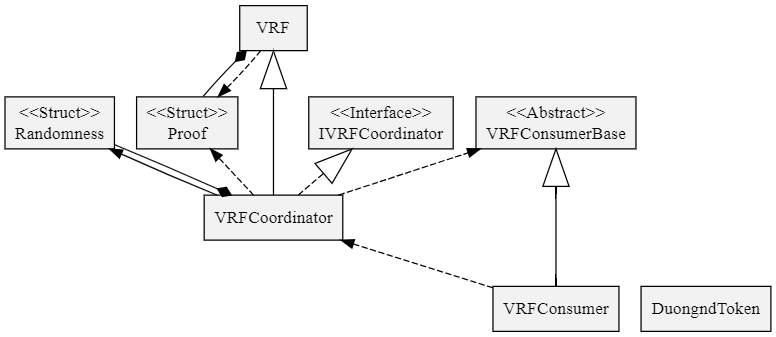
\includegraphics[scale = 0.5]{Figure/Overview.png}
    \caption{Thiết lớp hợp đồng thông minh}
    \label{fig:overview}
\end{figure}

Trong bảng \ref{table:structProof} thể hiện các thuộc tính trong Proof. Ngoài $pk,gamma,c,s,seed$ như trong thuật toán sinh số ngẫu nhiên có thể kiếm chứng trình bày trong chương \ref{chapter:Methodology} mỗi Proof sẽ chứa các bằng chứng của phép nhân vô hướng trên đường cong elliptic cũng như tổ hợp tuyến tính các điểm trên đường cong. Việc thêm các trường thông tin này giúp tránh phép nhân vô hướng thực hiện trên hợp đồng thông minh bằng cách sử dụng hàm ecrecover giả chữ ký được trình bày ở phụ lục \ref{appendix:B}.
\begin{table}[h!]
    \centering
    \begin{tabular}{||l l||}
    \hline
    \multicolumn{2}{c}{Proof}   \\
    \hline \hline
    pk          & uint256[2] \tab\\
    gamma       & uint256[2]\\
    c           & uint256   \\
    s           & uint256   \\
    seed        & uint256   \\
    uWitness    & address   \\
    cGammaWitness   &uint256[2]\\
    sHashWitness    &uint256[2]\\
    zInv            &uint256\\
    \hline
    \end{tabular}
    \caption{Struct Proof}
    \label{table:structProof}
\end{table}

Bảng \ref{table:structRandomness} thể hiện các trường thông tin của một kết quả ngẫu nhiên. Count thể hiện đã có bao nhiêu Oracle trả về bằng chứng hợp lệ đối với mỗi requestId của khách hàng. Khi đủ ngưỡng sẽ tự động trả về kết quả cho hợp đồng khách. 
\begin{table}[h!]
    \centering
    \begin{tabular}{||l l||}
    \hline
    \multicolumn{2}{c}{Randomness}   \\
    \hline \hline
    count           & uint256 \tab\\
    randomness      & uint256\\
    \hline
    \end{tabular}
    \caption{Struct Randomness}
    \label{table:structRandomness}
\end{table}

Bảng \ref{table:VRFCoordinator} thể hiện chi tiết hợp đồng xác thực. trong đó các trường thông tin sẽ được lưu trên storage EVM bao gồm:
\begin{enumerate}
    \item Owner: Người làm chủ hợp đồng, có quyền onlyOwner.
    \item DuongndToken: địa chỉ hợp đồng của đơn vị tiền.
    \item fee: Xác định chi phí mỗi lần hợp đồng khách yêu cầu dịch vụ.
    \item thresshold: ngưỡng số lượng các Oracle trung thực sẽ gửi kết quả về hợp đồng khách.
    \item Oracles: ánh xạ lưu lại các Oracle đã đăng ký thành công.
    \item isConsumer: ánh xạ lưu lại những hợp đồng khách đăng ký sử dụng dịch vụ.
    \item balances: số dư của hợp đồng khách hàng còn lại.
    \item nonces: ánh xạ lưu lại số các yêu cầu của mỗi khách hàng.
    \item requestIds: ánh xạ lưu lại kết quả ngẫu nhiên đối với mỗi requestId.
\end{enumerate}


\begin{table}[h!]
    \centering
    \begin{tabular}{||l||}
    \hline
    \multicolumn{1}{c}{VRFCoordinator}  \\
    \hline \hline
    Public:\\
    DuongndToken: ERC20\\
    owner: address\\
    fee: uint256\\
    threshold: uint256\\
    oracles: mapping(bytes32=>address)\\
    isConsumer: mapping(address=>bool)\\
    balances: mapping(address=>uint256)\\
    nonces: mapping(address=>uint256)\\
    requestIds: mapping(uint256=>Randomness)\\
    \hline
    Private:\\
    computeRequestId(uint256,sender): (uint256,uint256)\\
    External:\\
    registerOracle(address,uint256[2])\\
    Public:\\
    <<event>> RandomRequested(address, uint256, uint256) \tab\\
    <<event>> Transfer(address,address,uint256)\\
    <<modifier>> onlyOwner()\\
    constructor(address,uint256,uint256)\\
    hashOfKey(uint256[2]): bytes32\\
    fulfillRandomness(Proof,address)\\
    requestRandomness(): uint256\\
    addConsumer(address,uint256)\\
    removeConsumer(address)\\
    \hline
    \end{tabular}
    \caption{VRFCoordinator}
    \label{table:VRFCoordinator}
\end{table}

Đối với các phần logic của hợp đồng xác thực được lưu trong EVM code với các chức năng:
\begin{enumerate}
    \item computeRequestId: trả về requestId từ địa chỉ người gửi và số nonce.
    \item registerOracle: hàm cho phép đăng ký là một Oracle cung cấp dịch vụ.
    \item RandomRequested: sự kiện sẽ phát lên logs, cho biết đã khách hàng yêu cầu dịch vụ.
    \item onlyOwner: modifier hạn chế quyền chỉ cho owner.
    \item hashOfKey: hàm băm từ điểm trên đường cong về bytes32.
    \item fulfillRandomness: hàm sẽ được gọi từ Oracle trả về bằng chứng ngẫu nhiên.
    \item requestRandomness: hàm phát ra sự kiện yêu cầu số ngẫu nhiên.
    \item addConsumer: đăng ký sử dụng dịch vụ ngẫu nhiên cho khách hàng.
    \item removeConsumer: Xóa khách hàng khỏi danh sách được sử dụng dịch vụ.
\end{enumerate}

Một hợp đồng khách hàng đơn giản sử dụng dịch vụ sinh số ngẫu nhiên được thể hiện dưới bảng \ref{table:VRFConsumer}. Trong đó ta chỉ cần chỉ định hợp đồng VRFCoordinator thông qua địa chỉ. Cài đè hàm fulfillRandomness kế thừa từ hợp đồng trừu tương VRFConsumerBase (bảng \ref{table:VRFConsumerBase}) để lưu lại kết quả ngẫu nhiên. Cài đặt hàm requestRandomness để gửi yêu cầu số ngẫu nhiên.
\begin{table}[h!]
    \centering
    \begin{tabular}{||l||}
    \hline
    \multicolumn{1}{c}{VRFConsumer}  \\
    \hline \hline
    Public:\\
    vrfCoordinator: address\\
    randomNumber: uint256\\
    \hline
    Internal:\\
    fulfillRandomness(uint256,uint256)\tab\\
    Public:\\
    constructor()\\
    requestRandomness()\\
    \hline
    \end{tabular}
    \caption{VRFConsumer}
    \label{table:VRFConsumer}
\end{table}

\begin{table}[h!]
    \centering
    \begin{tabular}{||l||}
    \hline
    \multicolumn{1}{c}{VRFConsumerBase}  \\
    \hline \hline
    Private:\\
    vrfCoordinator: address\\
    \hline
    Internal:\\
    <<abstract>>fulfillRandomness(uint256,uint256)\tab\\
    External:\\
    rawFulfillRandomness(uint256,uint256)\\
    Public:
    constructor()\\
    \hline
    \end{tabular}
    \caption{VRFConsumerBase}
    \label{table:VRFConsumerBase}
\end{table}

Bảng \ref{table:VRF} mô tả hợp đồng VRF. Đây là hợp đồng có nhiệm vụ xác thực bằng chứng ngẫu nhiên và tính toán kết quả từ bằng chứng ngẫu nhiên này. VRF có các trường thuộc tính
\begin{enumerate}
    \item GROUP\_ORDER: bậc của đường cong secp256k1.
    \item FIELD\_SIZE: đặc số trường hữu hạn $F_p$.
    \item WORD\_LENGTH\_BYTES: độ dài của kiểu dữ liệu uint256.
    \item SQRT\_POWER: số mũ để tính căn bậc hai.\\
    Với $\text{SQRT\_POWER} = \frac{(\text{FIELD\_SIZE}+1)}{4}$\\
    $q = \text{FIELD\_SIZE}, q \equiv 3\mod{4}, x \equiv r^2 \mod{q}, \text{suy ra }x^{\text{SQRT\_POWER}} = \pm r \mod{q}$
    \item HASH\_TO\_CURVE\_HASH\_PREFIX: tiền tố thực hiện phép băm từ một số nguyên lớn tới một điểm trên đường cong.
    \item SCALAR\_FROM\_CURVE\_POINTS\_HASH\_PREFIX: tiền tố thực hiện phép băm từ một điểm trên đường cong tới một số nguyên lớn. 
    \item VRF\_RANDOM\_OUTPUT\_HASH\_PREFIX: tiền tố thực hiện phép băm từ bằng chứng hợp lệ ra kết quả ngẫu nhiên.
\end{enumerate}


\begin{table}[h!]
    \centering
    \begin{tabular}{||l||}
    \hline
    \multicolumn{1}{c}{VRF}  \\
    \hline \hline
    Private:\\
    GROUP\_ORDER\\
    FIELD\_SIZE\\
    WORD\_LENGTH\_BYTES\\
    SQRT\_POWER\\
    Internal:\\
    HASH\_TO\_CURVE\_HASH\_PREFIX\\
    SCALAR\_FROM\_CURVE\_POINTS\_HASH\_PREFIX \tab\\
    VRF\_RANDOM\_OUTPUT\_HASH\_PREFIX\\
    \hline
    Internal:\\
    bigModExp\\
    squareRoot\\
    ySquared\\
    isOnCurve\\
    fieldHash\\
    newCandidateSecp256k1Point\\
    hashToCurve\\
    ecmulVerify\\
    projectiveSub\\
    projectiveMul\\
    projectiveECAdd\\
    affineECAdd\\
    verifyLinearCombinationWithGenerator\\
    linearCombination\\
    scalarFromCurvePoints\\
    verifyVRFProof\\
    randomValueFromVRFProof\\
    \hline
    \end{tabular}
    \caption{VRF}
    \label{table:VRF}
\end{table}
Các hàm của hợp đồng VRF thể hiện trên bảng \ref{table:VRF} dùng để tính toán các phép tính trên đường cong Secp256k1 và xác thực bằng chứng ngẫu nhiên được gửi từ Oracle.
\begin{enumerate}
    \item bigModExp: hàm tính $\text{base}^{\text{e}} \mod{p}$.
    \item squareRoot: Hàm tính thử nghiệm căn bậc hai.
    \item isOnCurve: kiểm tra một cặp giá trị có là một điểm trên Secp256k1.
    \item fieldHash: hàm băm từ một bytes tới một số lớn thuộc $F_p$.
    \item newCandidateSecp256k1Point: Tính toán một cặp giá trị là ứng cử viên cho điểm trên đường cong.
    \item hashToCurve: hàm băm từ đầu vào tới một điểm trên đường cong.
    \item ecmulVerify: hàm xác thực phép nhân vô hướng trên đường cong.
    \item projectiveECAdd: cộng hai điểm trên đường cong với hệ tọa độ chiếu.
    \item affineECAdd: cộng hai điểm trên đường cong với hệ tọa độ affine.
    \item verifyLinearCombinationWithGenerator: Sử dụng kỹ thuật giả chữ ký xác thực kết quả tổ hợp tuyến một điểm trên đường cong với một phần tử sinh đường cong.
    \item linearCombination: xác thực kết quả tổ hợp tuyến tính hai điểm trên đường cong.
    \item scalarFromCurvePoints: hàm băm $H_3$ dựa trên hàm băm Keccak256. 
    \item verifyVRFProof: hàm xác thực bằng chứng ngẫu nhiên.
    \item randomValueFromVRFProof: hàm băm $H_2$ dựa trên hàm băm Keccak256.
\end{enumerate}
\subsection{Thiết kế lớp Oracle}
Với hệ thống trình bày trong đồ án, Oracle có hai nhiệm vụ chính. Thứ nhất đó là lắng nghe sự kiện trên nhật ký (logs) của blockchain. Thứ hai đó là mỗi khi nghe được sự kiện thì lập tức tính toán bằng chứng ngẫu nhiên rồi gửi tới cho hợp đồng xác thực VRFCoordinator.

Hình \ref{fig:oracleOverview} mô tả thiết kế của Oracle kế thừa lớp VRF và lớp Getlogs. Về cơ bản lớp VRF dùng để triển khai Oracle giống hệt hợp đồng VRF để triển khai VRFCoordinator.
\begin{figure}[h!]
    \centering
    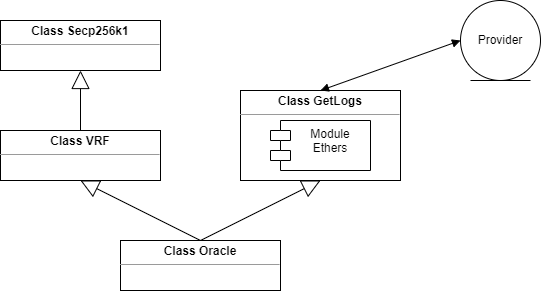
\includegraphics[scale = 0.7]{Figure/oracleOverview.png}
    \caption{Thiết kế Oracle}
    \label{fig:oracleOverview}
\end{figure}

Trong lớp Secp256k1 để xây dựng lên lớp VRF (bảng \ref{table:secp256k1}) có thuộc tính là các tham số công khai của đường cong Secp256k1. Các hàm chức năng với mục đích tính toán số lớn các điểm, tích vô hướng một số với một điểm dựa trên hai hệ tọa độ biểu diễn chiếu (projective) và hai chiều (affine).
\begin{table}[h!]
    \centering
    \begin{tabular}{||l||}
    \hline
    \multicolumn{1}{c}{Secp256k1}  \\
    \hline \hline
    Private:\\
    GROUP\_ORDER \tab \tab \tab \tab\\
    FIELD\_SIZE\\
    G\\
    PRIVATE\_KEY\\
    PUBLIC\_KEY\\
    \hline
    Internal:\\
    uint246\\
    mulmod\\
    addmod\\
    invmod\\
    projectiveAdd\\
    projectiveSub\\
    hashToCurve\\
    projectiveMul\\
    projectiveECAdd\\
    projectiveECMul\\
    affineECAdd\\
    affineECMul\\
    \hline
    \end{tabular}
    \caption{Lớp Secp256k xây dựng lên VRF}
    \label{table:secp256k1}
\end{table}





\begin{table}[h!]
    \centering
    \begin{tabular}{||l||}
    \hline
    \multicolumn{1}{c}{VRF}  \\
    \hline \hline
    Private:\\
    SQRT\_POWER\\
    PRIVATE\_KEY\\
    PUBLIC\_KEY\\
    Internal:\\
    HASH\_TO\_CURVE\_HASH\_PREFIX\\
    SCALAR\_FROM\_CURVE\_POINTS\_HASH\_PREFIX \tab\\
    VRF\_RANDOM\_OUTPUT\_HASH\_PREFIX\\
    \hline
    Internal:\\
    bigModExp\\
    squareRoot\\
    ySquared\\
    isOnCurve\\
    fieldHash\\
    newCandidateSecp256k1Point\\
    hashToCurve\\
    encodePacked\\
    addressFromPoint\\
    scalarFromCurvePoints\\
    vRF\\
    proofVRF\\
    \hline
    \end{tabular}
    \caption{Lớp VRF xây dựng lên Oracle}
    \label{table:VRFonOracle}
\end{table}

Khác ở chỗ hợp đồng VRF với mục đích xác thực bằng chứng ngẫu nhiên hơn nữa trong môi trường của Ethereum đã cài đặt sẵn đường cong Secp256k1. Về phía Oracle thì lớp VRF có chức năng sinh bằng chứng từ khóa bí mật. Do đó có chút khác biệt ở chức năng và các thuộc tính của lớp.
\begin{enumerate}
    \item $G$: phần tử sinh của đường cong.
    \item PUBLIC\_KEY: khóa công khai.
    \item PRIVATE\_KEY: khóa bí mật sinh số ngẫu nhiên
    \item addressFromPoint: hàm tính địa chỉ từ một điểm trên đường cong dựa trên thuật toán sinh địa chỉ của Ethereum.
    \item vRF: hàm tính bằng chứng ngẫu nhiên theo thuật toán VRF trình bày trong \ref{chapter:Methodology}.
    \item proofVRF: hàm tính bằng chứng ngẫu nhiên phù hợp với hợp đồng xác thực.
\end{enumerate}

Tổng quan lớp GetLogs được thể hiện ở bảng \ref{table:Getlogs}. Trong đó Module Ethers giúp Oracle kết nối với node trên mạng Ethereum. Lắng nghe sự kiện trên mỗi transaction thông qua chữ ký của sự kiện.
\begin{table}[H]
    \centering
    \begin{tabular}{||l||}
    \hline
    \multicolumn{1}{c}{GetLogs}  \\
    \hline \hline
    Private:\\
    pointer\\
    \hline
    Interal:\\
    parseLog \tab \tab \tab \tab\\
    \hline
    \end{tabular}
    \caption{Lớp Getlogs xây dựng lên Oracle}
    \label{table:Getlogs}
\end{table}
\subsection{Thử nghiệm}
Trong thử nghiệm thực tế, đồ án dùng các công nghệ được thể hiện trên bảng \ref{table:techuse}:
\begin{table}[H]
    \centering
    \begin{tabular}{||l l||}
    \hline
    \multicolumn{2}{c}{Công nghệ sử dụng}  \\
    \hline \hline
    Ví người dùng       & Metamask \tab \tab \tab\\
    Oracle              & Nodejs\\
    Hợp đồng thông minh & Solidity\\
    Kết nối với Node    & Influra\\
    Môi trường phát triển & Hardhat\\
    Mạng thử nghiệm         & Rinkeby\\
    Chuẩn tiền mã hóa       &ERC20\\
    \hline
    \end{tabular}
    \caption{Công nghệ sử dụng}
    \label{table:techuse}
\end{table}
Ngoài ra đồ án còn sử dụng thư viện:
\begin{enumerate}
    \item bn.js: thư viện tính toan số lớn trên nodejs.
    \item sol2uml: thư viện phục vụ mục đích vẽ biểu đồ lớp.
    \item openzeppelin/contracts: thư viện chuẩn ERC20.
    \item ethers: thư viện giúp kết nối với node Influra.
    \item chai: thư viện giúp việc kiểm thử code.
\end{enumerate}

Trong thử nghiệm đồ án, trình tự được thực hiện the trình tự:
\begin{enumerate}
    \item Triển khai đồng tiền thay thế (Alter token) đối với hệ thống theo chuẩn ERC20 của Oppenzepelin tại địa chỉ \\
    $0xFF6afB47AcB97A849ba51B20E57438d340EE8fbD$
    \item Địa chỉ triển khai đồng tiền ERC20 sẽ gửi một lượng tiền nhất định ERC20 tới cho hợp đồng khách hàng để phục vụ mục đích đăng ký dịch vụ.
    \item Các địa chỉ Oracle và khách hàng đều phải chưa một lượng tiền ETH (native token) để nhằm mục đích triển khai đăng ký.
    \item Triển khai hợp đồng điều phối VRFCoordinator tại địa chỉ\\
    $0xFE5725db462CC0a4ACa15FD9317298b1a52582b5$
    \item Đăng ký làm Oracle cho địa chỉ \\
    $0x45eFc65fF7e9ed85664924633416129Bc340Dcb8$
    \item Đăng ký Oracle cho địa chỉ \\
    $0x9Fb0dcaD42e3eBde8D1329a36A3F49dfbCE2141C$
    \item Triển khai hợp đồng khách hàng và yêu cầu số ngẫu nhiên.
    \item Đăng ký sử dụng dịch vụ sinh số ngẫu nhiên đối với hợp đồng khách.
\end{enumerate}
\section{Đánh giá}
Thử nghiệm cho thấy kết quả ngẫu nhiên được trả về trong thời gian nhanh nhất là 2 block. Thời gian mỗi block sẽ phụ thuộc vào từng mạng chuỗi khối có máy ảo Ethereum. Điều này sẽ là nhược điểm của hệ thống sinh số ngẫu nhiên có kiểm chứng bởi vì cần ít nhất một block để gửi yêu cầu và cần ít nhất một block để xác thực và gửi kết quả trả lại hợp đồng khách hàng. Đổi lại nhược điểm đó là hệ thống sẽ giảm rủi ro bị thao túng đi nhiều lần do mô hình phân tán của các Oracle.

Trong quá trình thực hiện, điều em tâm đắc nhất đó là đề xuất mô hình phân tán cho bên Oracle. Đây là một quá  trình khó khăn bởi vì việc tăng yêu cầu số lượng Oracle cho một yêu cầu ngẫu nhiên sẽ làm tăng một lượng chi phí cho yêu cầu. Hơn nữa việc cho phép đăng ký làm bên cung cấp dịch vụ sẽ phải có cơ chế phạt các Oracle không trung thực, hay bị từ chối dịch vụ,...Chưa kể tới khi có quá nhiều Oracle thì việc tăng số lượng nhà cung cấp dịch vụ sẽ khiến phần thường nhận được các bên cung cấp nhỏ. 

Điều tâm đắc trong quá trình thử nghiệm đó là thiết kế thuật toán lắng nghe sự kiện yêu cầu ngẫu nhiên cho các Oracle. Việc thiết kế này sẽ phải xem xét theo chữ ký sự kiện và được phát ra từ hợp đồng điều phối.
Sẽ có một con trỏ lưu lại chỉ dấu đã quét cho Oracle. Mỗi một chu kỳ (đảm bảo nhỏ hơn thời gian trung bình thợ đào công bố block mới) sẽ lấy dữ liệu một lần. Khi nghe được yêu cầu sẽ triển khai thuật toán VRF. Cũng mỗi chu kỳ này các Oracle sẽ xem xét các định danh yêu cầu trên hợp đồng thông minh, nếu quá 10 block mà yêu cầu chưa được thực hiện thì Oracle sẽ thực hiện điều này.
\end{document}